% Appendix: Cross-Dataset Robustness Results

\section{Cross-Dataset Robustness Results}
\label{app:cross_dataset_results}

\begin{figure}[H]
    \centering
    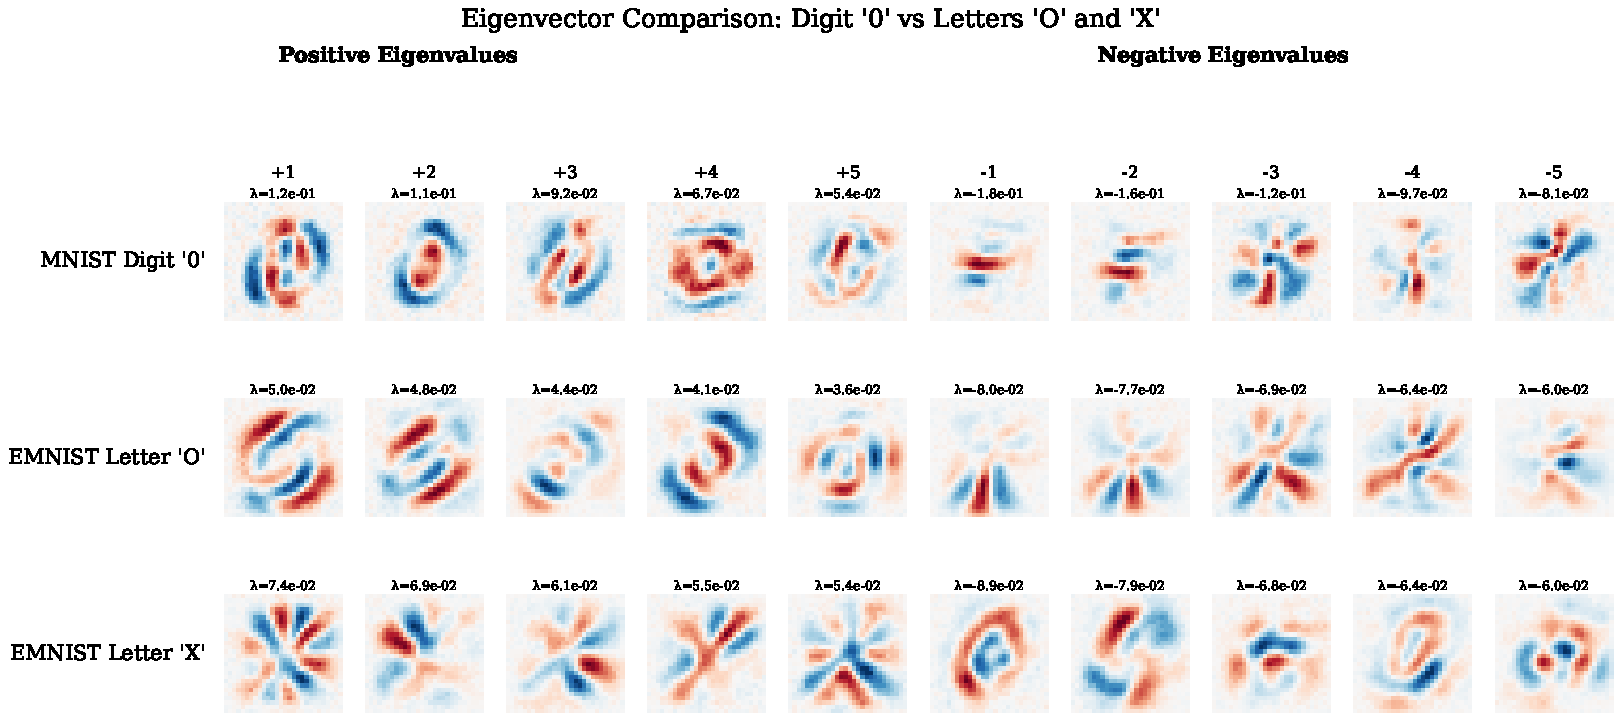
\includegraphics[width=0.9\linewidth]{figures/extension2/extension2_3way_comparison_0_O_X.pdf}
    \caption{Three-way eigenvector comparison: MNIST-0, EMNIST-O, and EMNIST-X. The top eigenvectors for each class are visually distinct from one another.}
    \label{fig:3way_comparison}
\end{figure}

\begin{table}[H]
\centering
\caption{Cross-Dataset Accuracy: MNIST $\leftrightarrow$ EMNIST-Digits (mean over 5 seeds).}
\label{tab:mnist_emnist_digits}
\small
\begin{tabular}{lc}
\toprule
\textbf{Direction} & \textbf{Accuracy} \\
\midrule
MNIST $\rightarrow$ EMNIST-Digits & 97.527 ± 0.024\% \\
EMNIST-Digits $\rightarrow$ MNIST & 97.910 ± 0.026\% \\
Bidirectional Average & 97.719 ± 0.012\% \\
\bottomrule
\end{tabular}
\end{table}

\begin{table}[H]
\centering
\caption{Cross-Dataset Accuracy: MNIST $\rightarrow$ USPS (mean over 5 seeds).}
\label{tab:usps}
\small
\begin{tabular}{lc}
\toprule
\textbf{Model} & \textbf{Accuracy} \\
\midrule
Baseline (no reg) & 53.42 ± 0.88\% \\
Regularized & 72.33 ± 0.83\% \\
\bottomrule
\end{tabular}
\end{table}

\begin{table}[H]
\centering
\caption{Letter$\to$Digit Transfer (regularized CoM model, 5 seeds).}
\label{tab:letter_digit}
\small
\begin{tabular}{lc}
\toprule
\textbf{Letter $\rightarrow$ Digit} & \textbf{Accuracy} \\
\midrule
O $\rightarrow$ 0 & 99.60 ± 0.05\% \\
I $\rightarrow$ 1 & 87.08 ± 0.10\% \\
Z $\rightarrow$ 2 & 88.75 ± 0.26\% \\
S $\rightarrow$ 5 & 87.38 ± 0.22\% \\
\bottomrule
\end{tabular}
\end{table}

\begin{figure}[H]
    \centering
    \begin{subfigure}{0.48\textwidth}
        \centering
        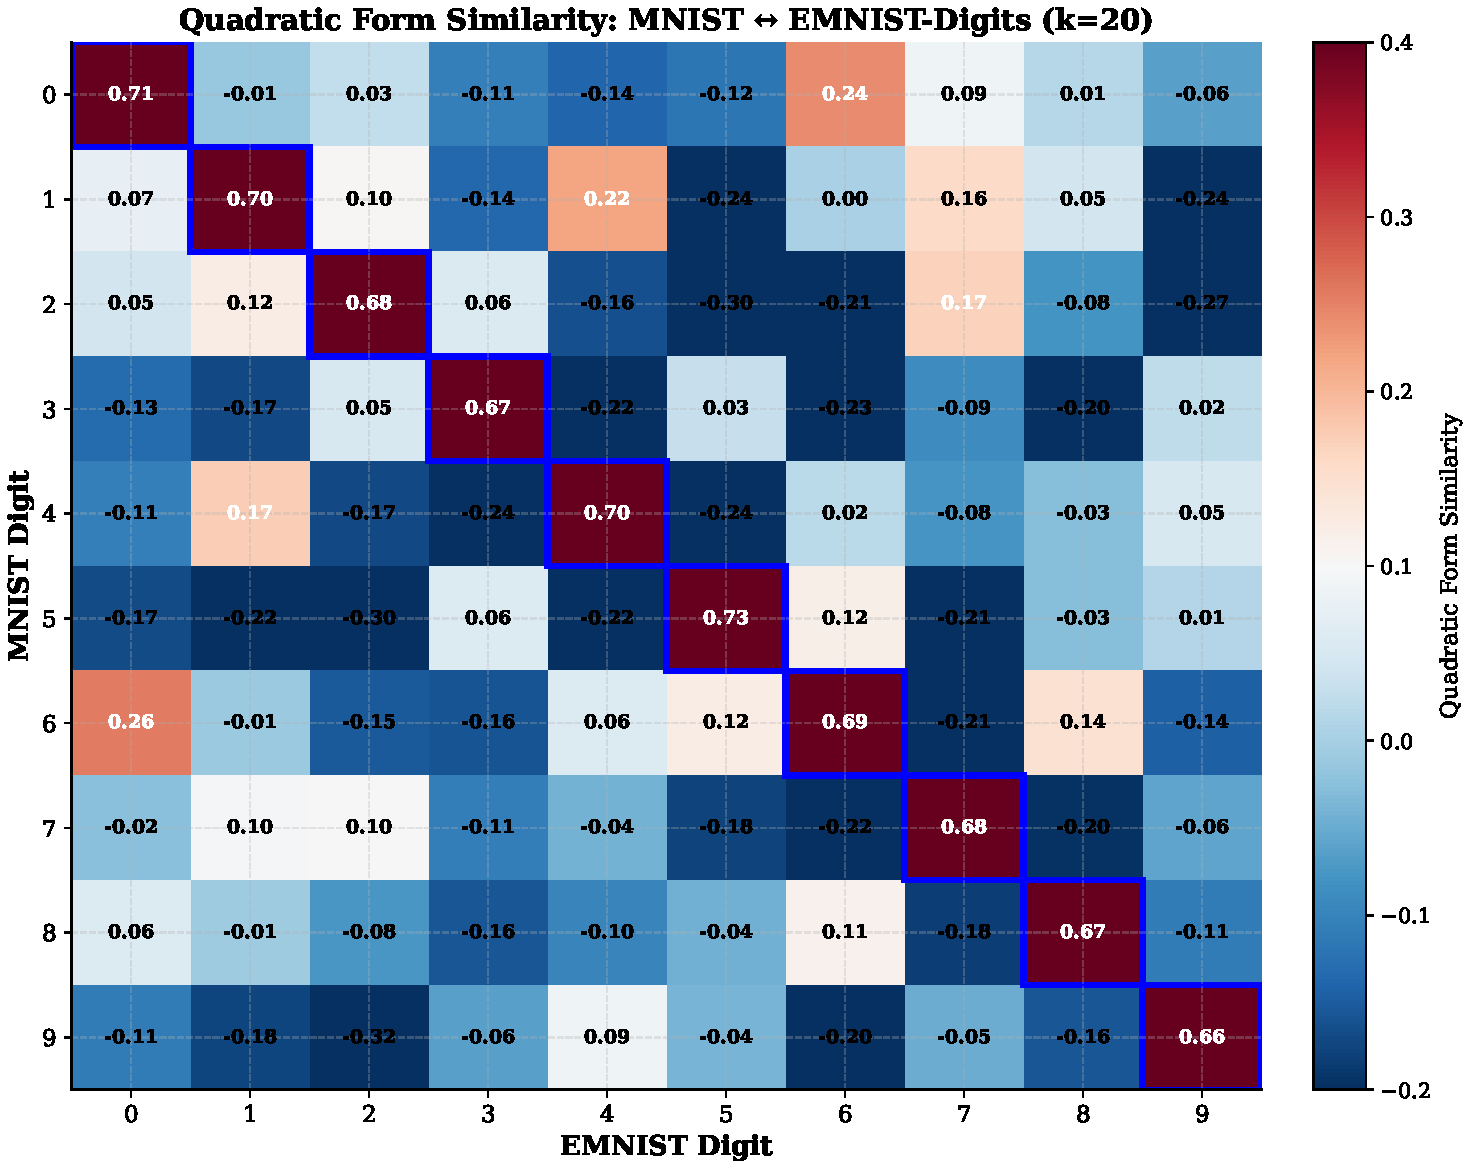
\includegraphics[height=4.5cm]{figures/extension2/extension2_quadratic_form_heatmap_digits.pdf}
        \caption{MNIST vs EMNIST-Digits}
        \label{fig:qf_digits}
    \end{subfigure}
    \hfill
    \begin{subfigure}{0.48\textwidth}
        \centering
        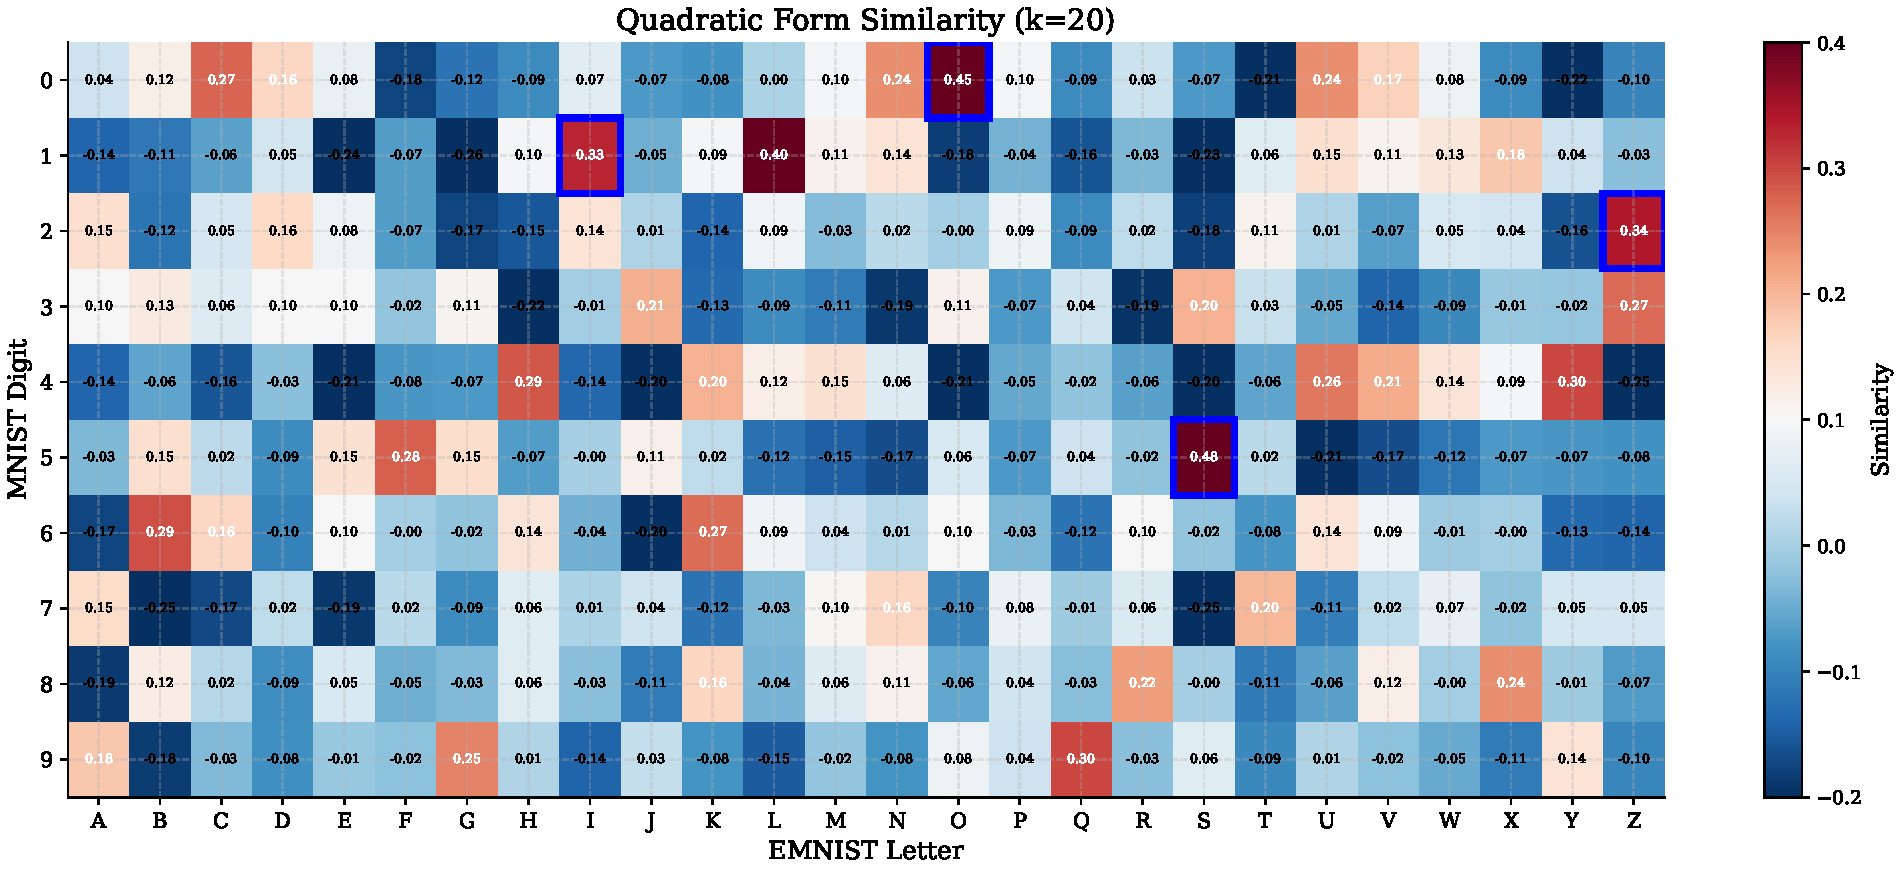
\includegraphics[height=4.5cm]{figures/extension2/extension2_heatmap_quadratic_form.pdf}
        \caption{MNIST vs EMNIST-Letters}
        \label{fig:qf_letters}
    \end{subfigure}
    \caption{Quadratic Form Similarity ($k=20$).
    (a) Strong diagonal confirms writer-independent circuits.
    (b) Bright entries at shape-matched pairs (0--O, 1--I, 2--Z, 5--S) indicate mechanistically similar circuits; unrelated pairs are near zero or negative.}
    \label{fig:quadratic_heatmaps}
\end{figure}

\begin{figure}[H]
    \centering
    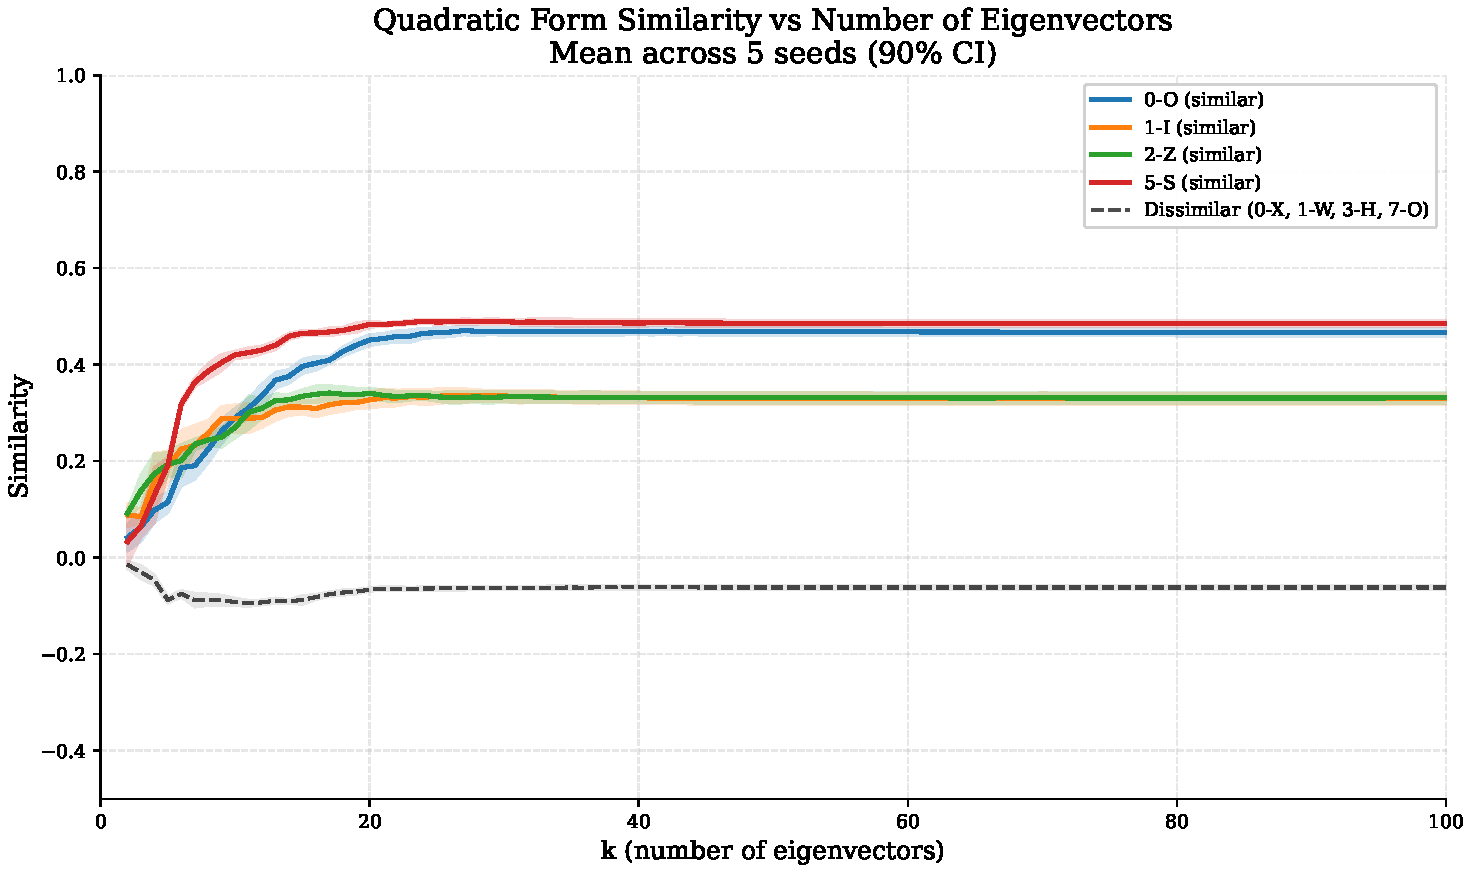
\includegraphics[width=0.7\linewidth]{figures/extension2/extension2_similarity_vs_k_quadratic_form.pdf}
    \caption{Quadratic Form Similarity vs number of eigenvectors $k$.
    Similar pairs converge around $k=20$; dissimilar pairs stay near zero with non-overlapping 90\% CIs.}
    \label{fig:similarity_vs_k}
\end{figure}

\begin{table}[H]
    \centering
    \caption{Ranking analysis: Position of expected letter among 26 EMNIST letters sorted by Quadratic Form Similarity. Random baseline: rank 13.}
    \label{tab:ranking_analysis}
    \small
    \begin{tabular}{lccccc}
        \toprule
        & 0--O & 1--I & 2--Z & 5--S & Mean \\
        \midrule
        Rank & \textbf{1} & \textbf{2} & \textbf{1} & \textbf{1} & \textbf{1.2} \\
        \bottomrule
    \end{tabular}
\end{table}
